\documentclass{article}

% todo
% forum analysis
  % zotero export quote and reference it in the text
  % make a csv to read the entire forum
  % check a way of analysing into multiple categories

% observable
  % quantify the forum posts by categories, do a sitemap

% Notes
% Citation commands \cite \parencite \textcite 

% Useful packages
\usepackage[a4paper,top=2cm,bottom=2cm,left=3cm,right=3cm,marginparwidth=1.75cm]{geometry}
\usepackage{amsmath}
\usepackage{graphicx}
\graphicspath{{images/}}
\usepackage{svg}
\svgsetup{inkscapelatex=false} % - does not use the latex fonts in imported svg

\usepackage{lmodern}
\usepackage{array}  % Allows for more flexible column formatting
\usepackage{booktabs}  % Improves table aesthetics
\usepackage[skip=0.5ex, justification=raggedright, singlelinecheck=false]{caption}
\usepackage{enumitem}
\usepackage{float} % Required for the H specifier
\usepackage{subcaption} % Required for sub-figures

% table
\usepackage{multirow}
\usepackage{tabularx}
\usepackage{booktabs}


\PassOptionsToPackage{colorlinks=true, allcolors=blue}{hyperref}
\usepackage[style=apa, backend=biber]{biblatex}

\addbibresource{main.bib}

\newcommand{\getyear}[1]{\citeyear{#1}}
\usepackage{hyperref}

\title{Building and Sustaining Open Source Art Communities: Lessons from the Processing Project}
\author{Tibor Udvari}

\begin{document}
\maketitle

\begin{abstract}
What are the dynamics that lead to the creation of a community around a piece of software? How do these dynamics influence the development of the software itself? This thesis explores these questions through the lens of the Processing community, a community of artists and designers who use the Processing software to create interactive art. The paper traces the history of the Processing community from its beginnings in 2001 to the present day, using a combination of interviews, archival research, and analysis of the software development cycle itself. The paper finds that the Processing community was created through a combination of factors, including the software's design, the community's shared values, and the community's shared history. The paper also finds that the community's shared history has influenced the development of the software itself, with the community's values and history influencing the software's design. The paper concludes by discussing the implications of these findings for the development of collaborative open source art software.
\end{abstract}

\newpage
%\tableofcontents

\section{Introduction}
% \subsection{The Background and Importance of Open Source Projects}
% -- about open source communities in general
% -- importance of open source projects, maybe mention how flash died out, and the recent unity price change ?

\subsection{The Processing Project: A brief overview}
% todo - adapt to focus more on the research question

Processing was developed as a programming language and environment specifically tailored for the media arts communities. Its inception took place at the MIT Media Lab's Aesthetics and Computation Group (ACG) in 2001, led by Ben Fry and Casey Reas. Its foundational concepts build upon the earlier work from the Design By Numbers (DBN) programming platform, a project spearheaded by John Maeda \parencite{fryModernPrometheusHistory2018}.

Ben Fry shed light on the holistic nature of the Processing initiative, noting:
\begin{quote}
"The processing project is a community, a piece of software that you run, and a language. And that order is important." – Ben Fry \parencite[19:22]{artsatmit2017CASTSymposium2017}
\end{quote}

In its design philosophy, Processing introduced the concept of "software sketches". It was designed with an accessible entry point for beginners, while also providing advanced capabilities for experienced users \parencite{reasProcessingProgrammingMedia2006}.

Over the years, Processing has been adopted across various disciplines, showcasing its versatility. To further its impact and development, the Processing Foundation was established, with notable contributors like Daniel Shiffman. The foundation aims to support and expand the reach of the Processing software and its associated projects.

\subsection{Objective and Scope of the Research}
% Choice of processing, because the community has been around for a while and the project is still alive and taught in schools, also at a high school level

% modular toolkit, not a monolith
% community, application, syntax
% commercial software

\section{Literature review}
\subsection{Open Source Contributions: Historical Perspective and Modern Implications}

Open source software has evolved from a grassroots, community-driven activity into a mainstream phenomenon influencing all sectors of software development. This transition has been analyzed from numerous perspectives, including Etienne Wenger's theory of Communities of Practice, which posits that learning occurs in social contexts \parencite{wengerCommunitiesPracticeLearning1998}. This theory underscores the importance of shared experiences, tools, and discourse in shaping a community's collective practice. In the context of open-source software, these dynamics offer invaluable insights into the sustainability and progression of such projects. For instance, the Processing community exemplifies more than just a collection of individual contributors; it represents a dynamic community molded by common goals and collective learning.

This communal focus contrasts sharply with the software development models described in Eric S. Raymond's seminal work "The Cathedral and the Bazaar" \parencite{CathedralBazaarMusings2002a}. The Cathedral model is marked by careful planning and centralized authority, more akin to the early GNU projects initiated by Richard Stallman in the 1980s. Conversely, the Bazaar model encourages open collaboration and decentralization—features commonly associated with contemporary open source projects. These two models can be conceptualized as endpoints of a continuum, with real-world communities of practice, like the Processing community, potentially embodying characteristics of both.

Although Richard Stallman's Free Software Movement initially utilized a Cathedral-like approach, the evolution of version control systems like Git has facilitated the adoption of more decentralized, Bazaar-like models. This technological and philosophical shift intriguingly complements Wenger's notions of "mutual engagement," "joint enterprise," and "shared repertoire"—elements that nurture a sense of community and shared objectives \parencite{wengerCommunitiesPracticeLearning1998}.

Fast-forwarding to today, the landscape now includes not just individual contributors but major corporations as well, injecting both challenges and opportunities into existing communities. The Processing project stands as a compelling case study to examine how an open-source community can preserve its foundational ethos while simultaneously adapting to contemporary requirements.

To holistically grasp the intricate interplay of social and technical factors contributing to the success of open-source initiatives, a multidimensional analysis is essential. Such an approach would synthesize various frameworks, including Wenger's Communities of Practice \parencite{wengerCommunitiesPracticeLearning1998} and Raymond's Cathedral and Bazaar models \parencite{CathedralBazaarMusings2002a}, aiming to provide a nuanced understanding of a community's past, present dynamics, and future potential.


\subsection{Motivations behind Open Source Contributions}
\subsection{The intersection of Creative Coding and Open Source}
%\subsection{Relevant Methodological Approaches in Computer Science and Anthropology}

\section{Methodology}

\subsection{Research Design}
Given the potential for memory bias due to the passage of time since the project's inception, this study employs a mixed-methods approach. While human memory can be fallible, introducing biases and even constructing false memories, quantitative analysis serves as a foundational component to mitigate these challenges. It allows for the identification of key contributors based on metrics such as commit frequency and significance, forum participation, and library contributions. These quantitative findings inform the selection of interviewees, acting as a preliminary filter to locate core contributors and library authors for qualitative interviews.

Anthropological studies have consistently highlighted the limitations of relying solely on quantitative data to understand the complex interplay of human experiences, beliefs, and emotions. Hence, qualitative interviews stand as a cardinal ethnographic instrument, offering access to the lived experiences, emic perspectives, and personal narratives of participants—dimensions that are often obscured in purely numerical representations.

By purposefully integrating quantitative methodologies with qualitative ethnographic approaches, this research aspires to offer a nuanced understanding of both the structural and phenomenological aspects of the Processing community.

\subsection{Quantitative Methods}
\subsubsection*{Data sources}

The research draws upon multiple data sources to form a comprehensive picture of the Processing community and its development practices. These range from forum discussions at various phases of the project to commit histories and issue trackers. The parsing status indicates the extent to which each data source has been prepared for analysis. 
\begin{table}[h]
    \raggedright
    \caption{Data sources}
    \label{table:data-sources}
    \begin{tabular}{l l l c}
        \toprule
        Name & Type & Status \\
        \midrule
        Processing alpha forum & Forum & Parsed \\
        Processing beta forum & Forum & Parsed  \\
        Processing 1.0 forum & Forum & Downloaded \\
        Processing 2.0 and 3.0 forum & Forum  & Not downloaded \\
        Current processing forum & Forum & Not downloaded\\
        Github project & Commit history & Parsed \\
        Processing Release Data & Release notes & Parsed \\
        Github Release Data & Release notes \& download statistics & Parsed \\
        Processing libraries\textsuperscript{*} & Software release information & Parsed \\

        \bottomrule
        \multicolumn{3}{l}{\footnotesize \textsuperscript{*}Note: The data set was reconstructed from the processing website archive and is not complete.}
    \end{tabular}
  \end{table}        

\subsubsection*{Evolution of Community Discussion Platforms}
In the early days of the Processing project, community interactions predominantly took place on forums. These forums served as a primary channel for users to share experiences, discuss problems, and seek help. Notably, the forum discussions underwent significant transformations in terms of platforms over the years, as can be observed in Table \ref{table:forums}. \parencite{ProcessingForum}

\begin{table}[h]
    \raggedright
    \caption{Archival forums composition}
    \label{table:forums}
    \begin{tabular}{l l l c}
        \toprule
        Forum name & Years & URL \\
        \midrule
        Processing alpha forum & 2002-2005 & \href{https://forum.processing.org/alpha/}{forum.processing.org/alpha} \\
        Processing beta forum & 2005-2010 & \href{https://forum.processing.org/beta/}{forum.processing.org/beta}  \\
        Processing 1.0 forum & 2010-2013 & \href{https://forum.processing.org/one/}{forum.processing.org/one} \\
        Processing 2.0 and 3.0 forum & 2013-2018 & \href{https://forum.processing.org/two/}{forum.processing.org/two} \\
        Current processing forum & 2018 - now & \href{https://discourse.processing.org/}{discourse.processing.org} \\
        \bottomrule
    \end{tabular}
  \end{table}

This dynamic shift from one platform to another indicates an evolving user-base and a growing set of needs and tools that community members require for effective collaboration.

\subsubsection*{Shift in Software-Related Discussions}

Initially, software-related discussions were confined to these forums. However, as the project matured, the complexity of issues warranted more specialized platforms for effective tracking and resolution. Consequently, the community transitioned from forums to Bugzilla \parencite{BugzillaArchiveProcessing} and eventually to GitHub Issues\parencite{ProcessingProcessingSource}\parencite{ProcessingProcessing4Processing}. 

\subsubsection*{The Ecosystem of Libraries}
An important milestone in the Processing ecosystem was the introduction of libraries. These libraries extended the functionalities of the base platform, thereby attracting a broader range of users and contributors. Such an analysis not only sheds light on the diversification of the project but also identifies key contributors and library authors who could potentially be sought out for qualitative interviews. The identification of these contributors adds another layer to our understanding of community participation.

\begin{figure}[h!] 
    \centering 
    \includesvg[pretex=\sffamily\fontsize{5.58pt}{8pt}\selectfont, width=1\textwidth, keepaspectratio]{images/figure-libraries.svg}
    \caption{Distribution of Libraries in the Processing Project}
    \label{figure:libraries}  
  \end{figure}


\subsubsection{Forum Textual Analysis: Approach and Tools}
%The research process began by manually reading the forum to identify themes and complemented with quantitative approaches. 
%todo forum composition

% todo
% check how much there is to read, estimate time
% relevance of the topics

\subsubsection{Forum Contributions Descriptive Statistics}

\subsection{Qualitative Methods}
\subsubsection{Interviews: Sample Selection, Interview Guide and Tools}
The introduction of libraries in the Processing ecosystem has served as a significant milestone, expanding the project's functionalities and, consequently, its user base. To gain nuanced insights into this aspect, our sample will be drawn from two main categories:

\begin{enumerate}
    \item \textbf{Core Contributors:} Those who have significantly contributed to the main Processing repository, shaping the foundational architecture.
    \item \textbf{Library Authors:} Contributors who have extended the functionalities of Processing by developing libraries, thus diversifying the ecosystem.
\end{enumerate}

These groups were identified through a combination of git commit history, contributions to the forums, and other public documentation. Special attention will be given to those who have been consistently active or have made impactful contributions.


\section{Data Presentation and Analysis}

\subsection{Quantitative Findings}

\subsubsection{Trends in Git Commits}

Considering the \textit{Processing} project, its dependency on its primary contributor, Ben Fry, stands out as a potential vulnerability. Fry's instrumental role over the past two decades underscores the significance of his contributions. Were they to be unexpectedly interrupted, the project could face substantial challenges. This scenario exemplifies a high bus factor risk \parencite{BusFactor2023}, wherein the success and continuity of a project are profoundly dependent on a single, or very few, contributors. Such vulnerabilities appear to be common in open source projects, a sentiment humorously captured in popular culture and comics \parencite{munroeDependency2020}.

\begin{figure}[h!] 
    \centering 
    \includesvg[pretex=\sffamily\fontsize{5.58pt}{8pt}\selectfont, width=1\textwidth, keepaspectratio]{images/figure-top12-github.svg}
    \caption{Top 12 source code contributors by number of commits}
    \label{fig:top12-github}  
  \end{figure}

\begin{figure}[h!] 
    \centering
    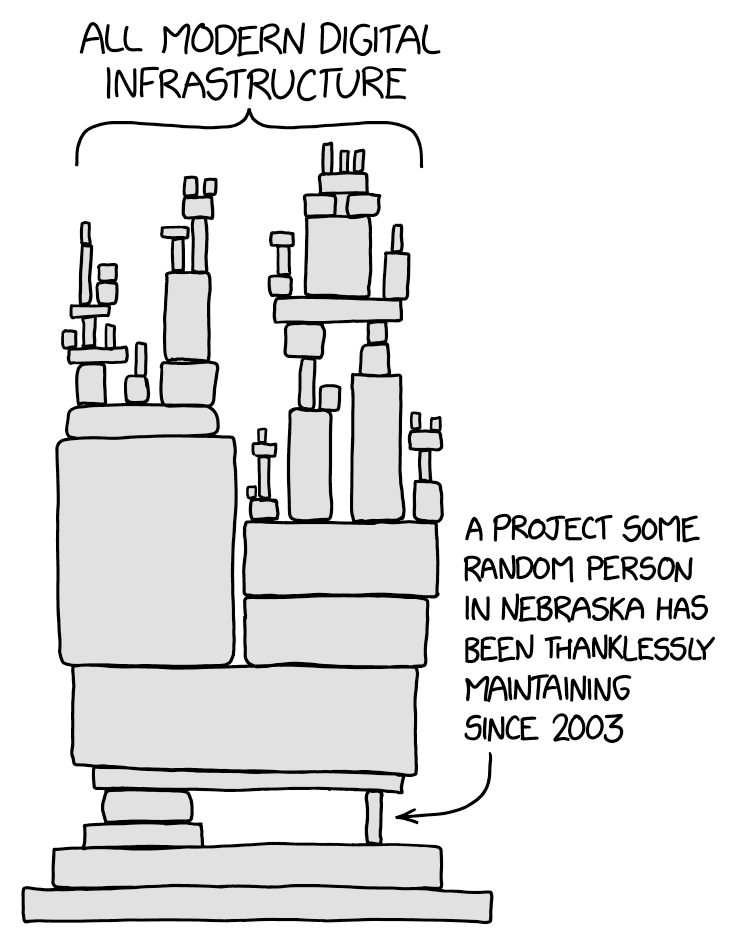
\includegraphics[width=0.5\textwidth]{dependency.png} 
    \caption{Dependency}
    \label{fig:dependency_comic}
    \small Source: \textit{XKCD}, \url{https://xkcd.com/2347/}, licensed under CC BY-NC 2.5.
\end{figure}

\subsubsection{Patterns in Forum Contributions}

Although Ben Fry remains the most active contributor in forum discussions, the activity distribution is more balanced compared to Git commits. This may be due to the broader range of topics discussed, including technical issues and bugs.

\begin{figure}[h!] 
    \centering 
    \includesvg[pretex=\sffamily\fontsize{5.58pt}{8pt}\selectfont, width=1\textwidth, keepaspectratio]{images/figure-forum-posts.svg}
    \caption{Top 12 authors by number of posts (Aggregated alpha and beta forum)}
    \label{fig:forum-posts}  
  \end{figure}

\begin{figure}[htbp] 
    \centering
    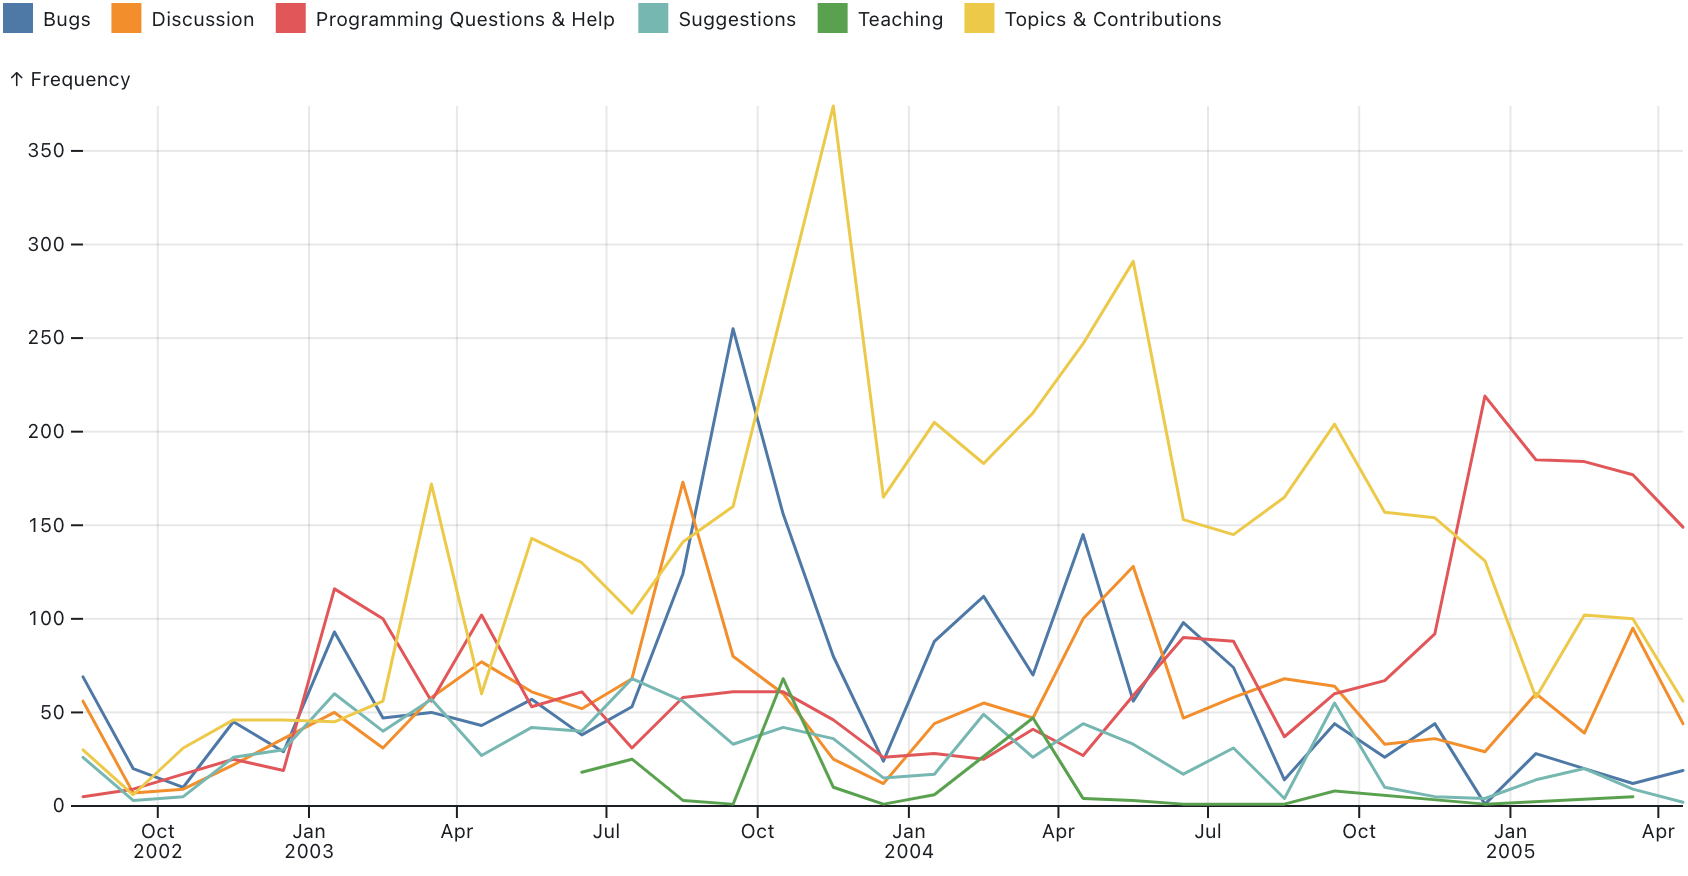
\includegraphics[width=1\textwidth]{alpha-forums-activity.png} 
    % \includesvg[pretex=\sffamily\fontsize{5.58pt}{8pt}\selectfont, width=0.6\textwidth]{images/alpha-forums-activity.svg}
    \caption{Forums activity}
    \label{fig:forum-activity}  
  \end{figure}

%\begin{figure}[h!] 
    \centering 
    \includesvg[pretex=\sffamily\fontsize{5.58pt}{8pt}\selectfont, width=1\textwidth, keepaspectratio]{images/figure-alltime-sourcecode-commits.svg}
    \caption{Top 25 source code contributors by number of commits}
    \label{fig:alltime-sourcecode-commits}  
  \end{figure}


%\begin{figure}[htbp] 
    \centering
    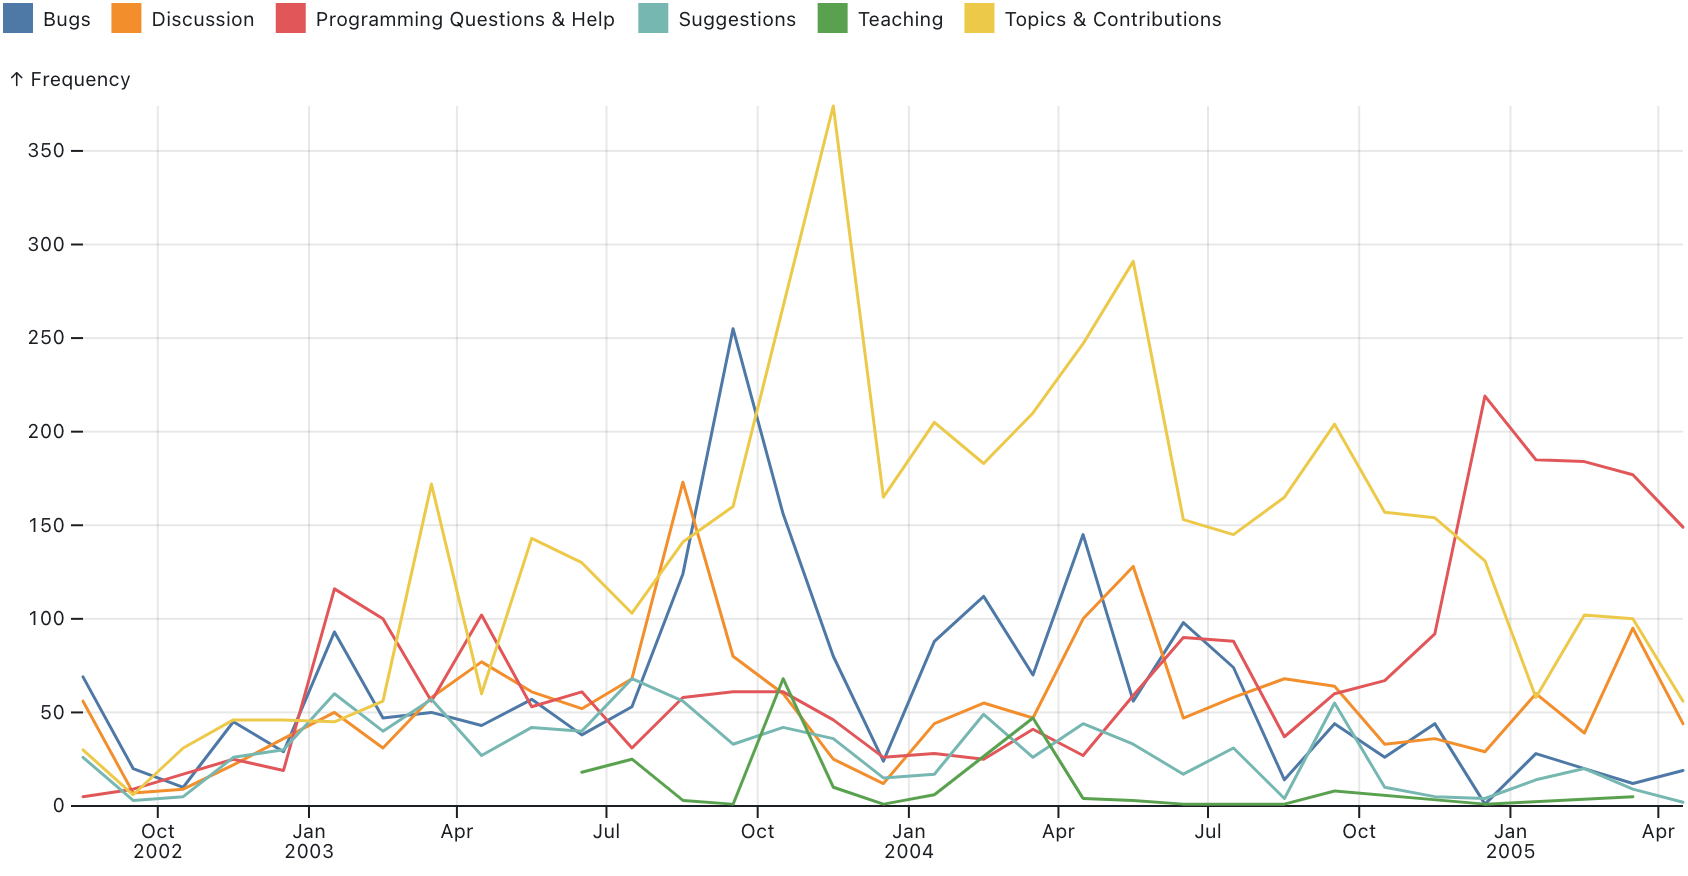
\includegraphics[width=1\textwidth]{alpha-forums-activity.png} 
    % \includesvg[pretex=\sffamily\fontsize{5.58pt}{8pt}\selectfont, width=0.6\textwidth]{images/alpha-forums-activity.svg}
    \caption{Forums activity}
    \label{fig:forum-activity}  
  \end{figure}


\subsubsection{Synthesized Data Analysis: Git Commits, Releases, and Forum Activity}

\begin{figure}[!htbp] 
    \centering 
    %\includesvg[pretex=\sffamily\fontsize{5.58pt}{8pt}\selectfont, width=1\textwidth, keepaspectratio]{images/figure-forum-git-activity.png}
    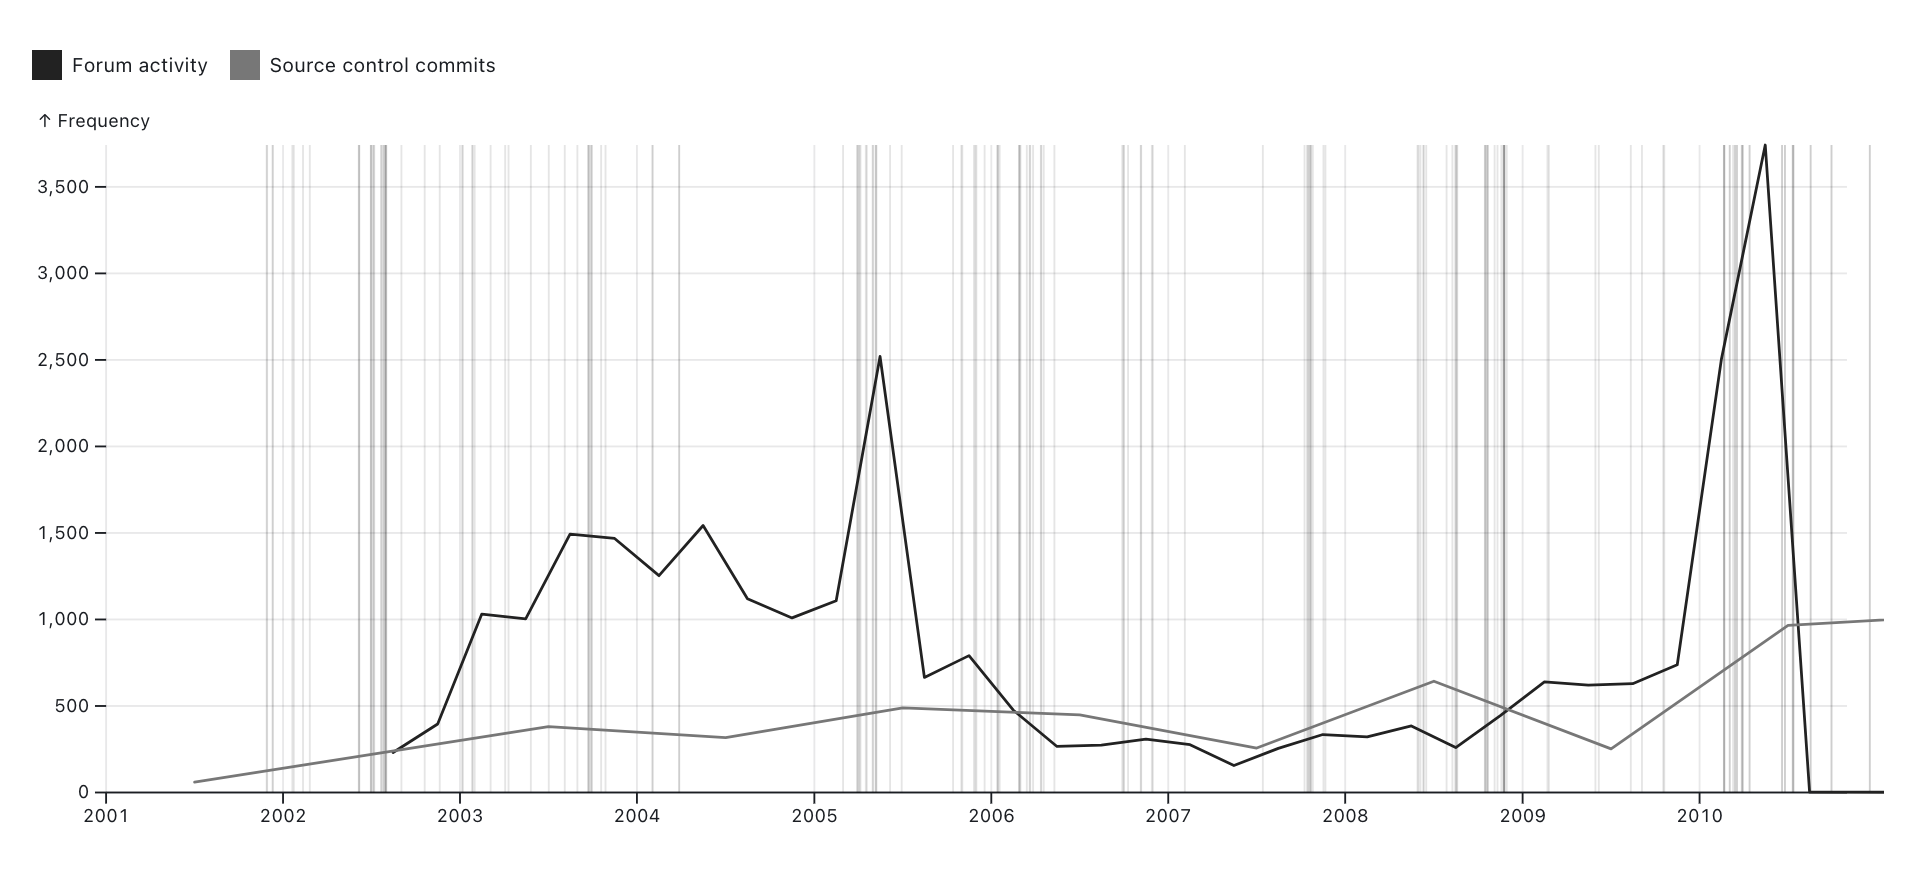
\includegraphics[width=1\textwidth]{images/figure-forum-git-activity.png} 

    \caption{Forum vs git activity vs releases (vertical lines)}
    \label{figure:forum-git-activity}  
  \end{figure}
\newpage
\subsubsection{Alpha Forum Patterns in Forum Contributions (to remove)}
There were 11,926 posts across 2,626 topics from 02/08/2002, 15:29 to the 19/04/2005, 09:55 across 1039 authors in the forum.

The alpha forum was a YaBB (Yet another Bulletin Board), it was seperated into forums which conained boards which contained topics which contained posts.

\begin{figure}
    \centering 
    \includesvg[pretex=\sffamily\fontsize{5.58pt}{8pt}\selectfont, width=1\textwidth, keepaspectratio]{images/alpha-forums-by-posts.svg}
    \caption{Topics by post number}
    \label{fig:forums}  
  \end{figure}

\subsection{Qualitative Insights}
\subsubsection{Themes from the Forum}
\subsubsection{Interview Highlights and Key Takeaways}

\section{Discussion}

\subsection{Integrating Quantitative and Qualitative Findings}
\subsection{Implications for the Open Source Community}
\subsection{The Unique Case of Processing and Creative Coding}
\subsection{Limitations of the Study}

\section{Conclusion and Recommendations}

\subsection{Recap of Key Findings}
\subsection{Practical Implications for Open Source Projects}
\subsection{Recommendations for Future Research}

\section{Acknowledgements}
I'm grateful to Randall Munroe of XKCD for his insightful and humorous comic strips. The comic "Dependency" from \getyear{munroeDependency2020} is in Figure~\ref{fig:dependency_comic} and cited as~\cite{munroeDependency2020}. It's under the Creative Commons Attribution-NonCommercial 2.5 License (CC BY-NC 2.5). License details: \url{https://creativecommons.org/licenses/by-nc/2.5/}.

\section{Bibliography}
\printbibliography

\section{Appendices}

\subsection{Interview Transcripts}

\section*{Interview Guide for Core Contributor}

\subsection*{Perceptions of Expertise and Community Role}

\begin{enumerate}
    \item Has your consistent involvement in resolving technical queries cultivated a sense of expertise or personal satisfaction for you?
    \item Can you comment on the emotional or psychological rewards, if any, you get from contributing?
    \item If you ceased your contributions tomorrow, what implications do you think that would have on the Processing project?
\end{enumerate}

\subsection*{Social Dynamics within the Community}

\begin{enumerate}[resume]
    \item How would you characterize the social fabric of the Processing community?
    \item Can you share an instance where the community's collective efforts resulted in something you alone couldn't have achieved?
    \item Have you ever experienced any conflicts within the community, and how were they resolved?
\end{enumerate}

\subsection*{Views on Technology and Development}

\begin{enumerate}[resume]
    \item What are your opinions on Flash and other proprietary technologies as they relate to Processing?
    \item Your contributions to Processing have been notably consistent. How do you interpret the fluctuating participation rates from others?
\end{enumerate}

\subsection*{Community and Open Source Development}

\begin{enumerate}[resume]
    \item What has been your observation regarding the community's growth, particularly concerning contributions to open source?
    \item Can you recall any "eureka moments" that significantly influenced the community's direction or ethos?
\end{enumerate}

\subsection*{Legacy and Continuation}

\begin{enumerate}[resume]
    \item How did p5 come into being as a continuation or evolution of Processing?
    \item What role did early literature play in legitimizing or boosting the project? Do you recall the impact of O'Reilly books or other publications?
\end{enumerate}

\section*{Interview Guide for Library Contributor}

\subsection*{Introduction and Motivation}

\begin{enumerate}
    \item What problem prompted you to contribute to Processing?
    \item How did you first hear about and decide to engage with the Processing community?
\end{enumerate}

\subsection*{Social Dynamics and Collaboration}

\begin{enumerate}[resume]
    \item Have you collaborated with other community members? What was that experience like?
    \item Were there any challenges in aligning your contributions with the broader community objectives?
\end{enumerate}
\subsection{Data Collection Tools and Scripts}

\begin{itemize}
    \item \href{https://forum.processing.org/alpha/}{Processing Alpha Forum}
    \item \href{https://observablehq.com/d/042b1cf42ea9bb5e}{Observable Notebook for Forum Analysis}
\end{itemize}


\subsection{List of Forum Threads Analyzed}


\end{document}